\begin{vd}\textbf{Prob1.5 IPhO 1996}\\
Hai dây dẫn thẳng rất dài không có từ tính $C_+$ và $C_-$ cách điện với nhau và mang dòng điện $I$ theo chiều dương và chiều âm của trục $z$. Tiết diện của dây dẫn (phần kẻ vạch trên hình) được giới hạn bởi các vòng tròn đường kính $D$ trên mặt phẳng $x - y$, các tâm cách nhau $\dfrac{D}{2}$. Tiết diện của mỗi dây là $\tron{\dfrac{1}{12}\pi + \dfrac{1}{8}\sqrt{3}}D^2$. Dòng điện trên mỗi dây dẫn được phân bố đều trên tiết diện.
\begin{center}
    

% Pattern Info
 
\tikzset{
pattern size/.store in=\mcSize, 
pattern size = 5pt,
pattern thickness/.store in=\mcThickness, 
pattern thickness = 0.3pt,
pattern radius/.store in=\mcRadius, 
pattern radius = 1pt}
\makeatletter
\pgfutil@ifundefined{pgf@pattern@name@_vjd2ozv2u}{
\pgfdeclarepatternformonly[\mcThickness,\mcSize]{_vjd2ozv2u}
{\pgfqpoint{0pt}{0pt}}
{\pgfpoint{\mcSize+\mcThickness}{\mcSize+\mcThickness}}
{\pgfpoint{\mcSize}{\mcSize}}
{
\pgfsetcolor{\tikz@pattern@color}
\pgfsetlinewidth{\mcThickness}
\pgfpathmoveto{\pgfqpoint{0pt}{0pt}}
\pgfpathlineto{\pgfpoint{\mcSize+\mcThickness}{\mcSize+\mcThickness}}
\pgfusepath{stroke}
}}
\makeatother

% Pattern Info
 
\tikzset{
pattern size/.store in=\mcSize, 
pattern size = 5pt,
pattern thickness/.store in=\mcThickness, 
pattern thickness = 0.3pt,
pattern radius/.store in=\mcRadius, 
pattern radius = 1pt}
\makeatletter
\pgfutil@ifundefined{pgf@pattern@name@_obejvprpe}{
\pgfdeclarepatternformonly[\mcThickness,\mcSize]{_obejvprpe}
{\pgfqpoint{0pt}{0pt}}
{\pgfpoint{\mcSize+\mcThickness}{\mcSize+\mcThickness}}
{\pgfpoint{\mcSize}{\mcSize}}
{
\pgfsetcolor{\tikz@pattern@color}
\pgfsetlinewidth{\mcThickness}
\pgfpathmoveto{\pgfqpoint{0pt}{0pt}}
\pgfpathlineto{\pgfpoint{\mcSize+\mcThickness}{\mcSize+\mcThickness}}
\pgfusepath{stroke}
}}
\makeatother
\tikzset{every picture/.style={line width=0.75pt}} %set default line width to 0.75pt        

\begin{tikzpicture}[x=0.75pt,y=0.75pt,yscale=-1,xscale=1]
%uncomment if require: \path (0,449); %set diagram left start at 0, and has height of 449

%Straight Lines [id:da6867445708340851] 
\draw    (168,206.26) -- (409.51,206.26) ;
\draw [shift={(412.51,206.26)}, rotate = 180] [fill={rgb, 255:red, 0; green, 0; blue, 0 }  ][line width=0.08]  [draw opacity=0] (10.72,-5.15) -- (0,0) -- (10.72,5.15) -- (7.12,0) -- cycle    ;
%Straight Lines [id:da6324801988556674] 
\draw    (290.26,327.7) -- (290.26,87.82) ;
\draw [shift={(290.26,84.82)}, rotate = 450] [fill={rgb, 255:red, 0; green, 0; blue, 0 }  ][line width=0.08]  [draw opacity=0] (10.72,-5.15) -- (0,0) -- (10.72,5.15) -- (7.12,0) -- cycle    ;
%Shape: Path Data [id:dp3402301434882209] 
\draw  [pattern=_vjd2ozv2u,pattern size=6pt,pattern thickness=0.75pt,pattern radius=0pt, pattern color={rgb, 255:red, 0; green, 0; blue, 0}] (258.47,142.44) .. controls (270.04,142.44) and (280.9,145.52) .. (290.26,150.91) .. controls (271.12,161.93) and (258.23,182.59) .. (258.23,206.26) .. controls (258.23,229.93) and (271.12,250.59) .. (290.26,261.61) .. controls (280.9,266.99) and (270.04,270.07) .. (258.47,270.07) .. controls (223.23,270.07) and (194.65,241.5) .. (194.65,206.26) .. controls (194.65,171.01) and (223.23,142.44) .. (258.47,142.44) -- cycle ;
%Shape: Path Data [id:dp07808342622314401] 
\draw  [pattern=_obejvprpe,pattern size=6pt,pattern thickness=0.75pt,pattern radius=0pt, pattern color={rgb, 255:red, 0; green, 0; blue, 0}] (322.04,270.07) .. controls (310.47,270.07) and (299.62,266.99) .. (290.26,261.61) .. controls (309.4,250.59) and (322.29,229.93) .. (322.29,206.26) .. controls (322.29,182.59) and (309.4,161.93) .. (290.26,150.91) .. controls (299.62,145.52) and (310.47,142.44) .. (322.04,142.44) .. controls (357.29,142.44) and (385.86,171.01) .. (385.86,206.26) .. controls (385.86,241.5) and (357.29,270.07) .. (322.04,270.07) -- cycle ;

% Text Node
\draw (170.52,207.44) node [anchor=north west][inner sep=0.75pt]    {$C_{+}$};
% Text Node
\draw (387.09,207.44) node [anchor=north west][inner sep=0.75pt]    {$C_{-}$};
% Text Node
\draw (416.29,207.62) node [anchor=north west][inner sep=0.75pt]    {$x$};
% Text Node
\draw (272.03,77.22) node [anchor=north west][inner sep=0.75pt]    {$y$};
\end{tikzpicture}
\end{center}
Xác định từ trường $B (x,y)$ trong khoảng không gian giữa hai dây dẫn.
\end{vd}
\begin{loigiai}\\
Khoảng không gian giữa hai dây dẫn không có dòng điện chạy qua có thể xem như có sự chồng chất của hai dòng điện độ lớn như nhau và ngược chiều. Mỗi dây dẫn hình trụ phải mang dòng điện $I'$ lớn hơn dóng điện $I$ mang bởi tiết diện thật sự của nó (hình mặt trăng). Tỉ số  giữa dòng điện $I$ và $I'$ bằng tỉ số giữa hai tiết diện.
\[\dfrac{I}{I'} = \dfrac{\tron{\dfrac{1}{12}\pi + \dfrac{1}{8}\sqrt{3}}D^2}{4\pi D^2} = \dfrac{2\pi + 3\sqrt{3}}{6\pi}.\]
Áp dụng định luật Ampère, từ trường do dây dẫn hình trụ gây ra tại điểm cách dây đoạn $r$ và nằm bên trong dây dẫn là
\[B_\phi = \dfrac{\mu_0}{2\pi r} \dfrac{\pi r^2}{\dfrac{\pi}{4}D^2}I' = \dfrac{2\mu_0I'r}{\pi D^2}.\]
Các thành phần của từ trường này là
\[\heva{B_x &= - B_\phi \dfrac{y}{r} =  - \dfrac{2\mu_0I'y}{\pi D^2} \\ B_y &= B_\phi \dfrac{x}{r} = \dfrac{2\mu_0I'x}{\pi D^2}}.\]
Đối với phần chồng chất từ trường, các dòng điện $\pm I'$ và các hình trụ tương ứng có tâm nằm ở $x = \mp \dfrac{D}{4}$.\\
Thành phần từ trường tổng hợp theo phương $x$ sẽ bị triệt tiêu, thành phần từ trường theo phương $y$ là:
\[B_y = \dfrac{2\mu_0}{\pi D^2} \tron{I'\tron{x + \dfrac{D}{4}} - I'\tron{x - \dfrac{D}{4}}} = \dfrac{\mu_0I'}{\pi D} = \dfrac{6\mu_0I}{\tron{2\pi + 3\sqrt{3}}D}.\]
Từ trường này đều và hướng theo chiều dương trục $y$.
\end{loigiai}
\begin{vd}\textbf{Prob2 IPhO 1996}\\
Khoảng không gian giữa một cặp vật dẫn hình trụ đồng trục đã được rút chân không. Bán kính hình trụ trong là $a$, bán kính trong của hình trụ ngoài là $b$ như hình vẽ. Hình trụ ngoài gọi là anode và có thể đặt ở điện thế dương $V$ so với hình trụ trong. Người ta thiết lập một từ trường không đổi, đồng nhất $\ot{B}$ song song với trục hình trụ và hướng từ mặt hình vẽ lên phía trên. Bỏ qua các điện tích cảm ứng trên các vật dẫn.
\begin{center}
    

% Pattern Info
 
\tikzset{
pattern size/.store in=\mcSize, 
pattern size = 5pt,
pattern thickness/.store in=\mcThickness, 
pattern thickness = 0.3pt,
pattern radius/.store in=\mcRadius, 
pattern radius = 1pt}
\makeatletter
\pgfutil@ifundefined{pgf@pattern@name@_rdtogkbx5}{
\pgfdeclarepatternformonly[\mcThickness,\mcSize]{_rdtogkbx5}
{\pgfqpoint{0pt}{-\mcThickness}}
{\pgfpoint{\mcSize}{\mcSize}}
{\pgfpoint{\mcSize}{\mcSize}}
{
\pgfsetcolor{\tikz@pattern@color}
\pgfsetlinewidth{\mcThickness}
\pgfpathmoveto{\pgfqpoint{0pt}{\mcSize}}
\pgfpathlineto{\pgfpoint{\mcSize+\mcThickness}{-\mcThickness}}
\pgfusepath{stroke}
}}
\makeatother

% Pattern Info
 
\tikzset{
pattern size/.store in=\mcSize, 
pattern size = 5pt,
pattern thickness/.store in=\mcThickness, 
pattern thickness = 0.3pt,
pattern radius/.store in=\mcRadius, 
pattern radius = 1pt}
\makeatletter
\pgfutil@ifundefined{pgf@pattern@name@_wjai8lwg3}{
\pgfdeclarepatternformonly[\mcThickness,\mcSize]{_wjai8lwg3}
{\pgfqpoint{0pt}{-\mcThickness}}
{\pgfpoint{\mcSize}{\mcSize}}
{\pgfpoint{\mcSize}{\mcSize}}
{
\pgfsetcolor{\tikz@pattern@color}
\pgfsetlinewidth{\mcThickness}
\pgfpathmoveto{\pgfqpoint{0pt}{\mcSize}}
\pgfpathlineto{\pgfpoint{\mcSize+\mcThickness}{-\mcThickness}}
\pgfusepath{stroke}
}}
\makeatother
\tikzset{every picture/.style={line width=0.75pt}} %set default line width to 0.75pt        

\begin{tikzpicture}[x=0.75pt,y=0.75pt,yscale=-1,xscale=1]
%uncomment if require: \path (0,428); %set diagram left start at 0, and has height of 428

%Shape: Ellipse [id:dp23326337030165578] 
\draw  [pattern=_rdtogkbx5,pattern size=6pt,pattern thickness=0.75pt,pattern radius=0pt, pattern color={rgb, 255:red, 0; green, 0; blue, 0}] (298.06,166.42) .. controls (298.06,153.89) and (308.22,143.73) .. (320.75,143.73) .. controls (333.28,143.73) and (343.44,153.89) .. (343.44,166.42) .. controls (343.44,178.95) and (333.28,189.11) .. (320.75,189.11) .. controls (308.22,189.11) and (298.06,178.95) .. (298.06,166.42) -- cycle ;
%Shape: Path Data [id:dp6743627958607954] 
\draw  [color={rgb, 255:red, 0; green, 0; blue, 0 }  ,draw opacity=0 ][pattern=_wjai8lwg3,pattern size=6pt,pattern thickness=0.75pt,pattern radius=0pt, pattern color={rgb, 255:red, 0; green, 0; blue, 0}] (320.75,88.26) .. controls (363.91,88.26) and (398.9,123.25) .. (398.9,166.42) .. controls (398.9,209.58) and (363.91,244.57) .. (320.75,244.57) .. controls (277.59,244.57) and (242.6,209.58) .. (242.6,166.42) .. controls (242.6,123.25) and (277.59,88.26) .. (320.75,88.26) -- cycle (214.17,166.42) .. controls (214.17,225.28) and (261.89,273) .. (320.75,273) .. controls (379.61,273) and (427.33,225.28) .. (427.33,166.42) .. controls (427.33,107.55) and (379.61,59.83) .. (320.75,59.83) .. controls (261.89,59.83) and (214.17,107.55) .. (214.17,166.42) -- cycle ;
%Shape: Ellipse [id:dp2698487761040751] 
\draw   (242.25,166.77) .. controls (242.25,123.41) and (277.39,88.26) .. (320.75,88.26) .. controls (364.11,88.26) and (399.25,123.41) .. (399.25,166.77) .. controls (399.25,210.12) and (364.11,245.27) .. (320.75,245.27) .. controls (277.39,245.27) and (242.25,210.12) .. (242.25,166.77) -- cycle ;
%Straight Lines [id:da5084734289815698] 
\draw    (320.75,166.77) -- (335.03,152.48) ;
\draw [shift={(337.16,150.36)}, rotate = 495] [fill={rgb, 255:red, 0; green, 0; blue, 0 }  ][line width=0.08]  [draw opacity=0] (10.72,-5.15) -- (0,0) -- (10.72,5.15) -- (7.12,0) -- cycle    ;
%Straight Lines [id:da47796361970572887] 
\draw    (320.75,166.42) -- (268.02,113.69) ;
\draw [shift={(265.9,111.56)}, rotate = 405] [fill={rgb, 255:red, 0; green, 0; blue, 0 }  ][line width=0.08]  [draw opacity=0] (10.72,-5.15) -- (0,0) -- (10.72,5.15) -- (7.12,0) -- cycle    ;
%Shape: Circle [id:dp2356750479628158] 
\draw   (310,218.5) .. controls (310,212.7) and (314.7,208) .. (320.5,208) .. controls (326.3,208) and (331,212.7) .. (331,218.5) .. controls (331,224.3) and (326.3,229) .. (320.5,229) .. controls (314.7,229) and (310,224.3) .. (310,218.5) -- cycle ;
%Shape: Circle [id:dp023767196122381984] 
\draw  [fill={rgb, 255:red, 0; green, 0; blue, 0 }  ,fill opacity=1 ] (317.14,218.5) .. controls (317.14,216.64) and (318.64,215.14) .. (320.5,215.14) .. controls (322.36,215.14) and (323.86,216.64) .. (323.86,218.5) .. controls (323.86,220.36) and (322.36,221.86) .. (320.5,221.86) .. controls (318.64,221.86) and (317.14,220.36) .. (317.14,218.5) -- cycle ;

% Text Node
\draw (275.6,139.39) node [anchor=north west][inner sep=0.75pt]    {$b$};
% Text Node
\draw  [color={rgb, 255:red, 255; green, 255; blue, 255 }  ,draw opacity=0 ][fill={rgb, 255:red, 255; green, 255; blue, 255 }  ,fill opacity=0 ]  (327.95,157.57) -- (345.95,157.57) -- (345.95,181.57) -- (327.95,181.57) -- cycle  ;
\draw (327,164.57) node [anchor=north west][inner sep=0.75pt]    {$a$};
% Text Node
\draw (292.5,204.9) node [anchor=north west][inner sep=0.75pt]    {$\ot{B}$};
\end{tikzpicture}
\end{center}
Trong bài này ta nghiên cứu động lực học của electron khối lượng nghỉ ${m}$, tích điện $-e$. Các electron này phát ra từ bề mặt của hình trụ trong.
\begin{enumerate}[1)]
    \item Thoạt đầu ta đặt điện thế $V$ nhưng $\ot{B} = 0$. Các electron được giải phóng từ mặt khối trụ trong với vận tốc không đáng kể. Hãy tính tốc độ của nó khi nó đập vào anode: cho kết quả trong hai trường hợp phi tương đối tính và tương đối tính.\\
\end{enumerate}

    Trong các phần còn lại của bài toán chỉ cần xét trường hợp phi tương đối tính.\\
    \begin{enumerate}[1)]
    \setcounter{enumi}{1}
    \item Bây giờ cho $V =0 $ và cho tác dụng của từ trường $\ot{B}$. Một electron phát ra theo phương bán kính với vận tốc $\ot{v}_{0}$. Khi từ trường lớn hơn một giá trị tới hạn $B_{c}$, electron không tới được anode. Vẽ quỹ đạo của electron khi $B$ hơi lớn hơn $B_{c}$.\\
\end{enumerate}
    Từ đây về sau ta cho tác dụng đồng thời của $V$ và từ trường đồng nhất $\ot{B}$.\\
    \begin{enumerate}[1)]
    \setcounter{enumi}{2}
    \item Từ trường sẽ gây ra cho electron một moment động lượng $L$ khác không đối với trục hình trụ. Hãy viết phương trình thể hiện tốc độ biến thiên $\dfrac{\dd L}{\dd t}$ của moment động lượng. Chứng minh rằng phương trình đó nói lên đại lượng \[L - keBr^2\] không thay đổi trong suốt quá trình chuyển động, trong đó $k$ là một số xác định không có thứ nguyên, $r$ là khoảng cách tính đến trục hình trụ. Xác định giá trị của $k$.
    \item Xét một electron phát ra từ hình trụ trong với tốc độ không đáng kể và không đến được anode, nhưng đạt được khoảng cách tối đa $r_m$ đối với trục hình trụ. Xác định tốc độ $v$ tại điểm mà khoảng cách theo phương bán kính là lớn nhất theo $r_{m}$.
    \item Chúng ta muốn dùng từ trường để điều khiển dòng electron tới anode. Với $B$ lớn hơn từ trường tới hạn $B_{c}$, thì electron phát ra từ bề mặt khối trụ trong với tốc độ không đáng kể sẽ không đến được anode. Xác định ${B}_{{c}}$. 
    \item Nếu electron được phát ra bằng cách đốt nóng khối trụ trong thì chúng có thể có tốc độ khác không ở bề mặt khối trụ trong. Thành phần vận tốc ban đầu song song với $\ot{B}$ là $v_{B}$, thành phần vuông góc với $\overrightarrow{{B}}$ là ${v}_{r}$ (theo phương bán kính) và ${v}_{\varphi}$ (theo phương vuông góc với bán kính). Hãy xác định từ trường tới hạn để electron đạt tới anode trong điều kiện như vậy.
\end{enumerate}
\end{vd}
\begin{loigiai}
\begin{enumerate}[1)]
    \item Thế năng mà electron nhận được $eV$ chuyển thành động năng.
    \[\dfrac{1}{2}mv^2 = eV, \qquad \text{(phi tương đối tính)} \]
    \[\dfrac{mc^2}{\sqrt{1 -\dfrac{v^2}{c^2}}} - mc^2 = eV. \qquad \text{(tương đối tính)}\]
    Do đó
    \[v = \heva{\sqrt{\dfrac{2eV}{m}}, \qquad \text{(phi tương đối tính)} \\ c\sqrt{1 - \tron{\dfrac{mc^2}{mc^2 + eV}}^2}. \qquad \text{(tương đối tính)}} \tag{1}\label{q.7.1}\]
    \item Khi $V = 0$, electron chuyển động trong từ trường đều, quỹ đạo của hạt là đường tròn. Vận tốc ban đầu có phương tiếp tuyến với đường tròn. \\
    Bán kính của quỹ đạo (hay còn gọi là bán kính cyclotron) xác định bằng phương trình cân bằng lực: lực Lorentz bằng lực hướng tâm
    \[eBv_0 = \dfrac{mv_0^2}{R} \rt B = \dfrac{mv_0}{eR}. \tag{2}\label{q.7.2}\]
    Từ hình vẽ, ta suy ra trong trường hợp tới hạn, bán kính $R$ của đường tròn phải thỏa mãn:
    \[\sqrt{a^2 + R^2} = b - R. \]
    Bình phương hai vế rồi biến đổi, ta được
    \[R = \dfrac{b^2 - a^2}{2b}.\]
    Thay giá trị của $R$ vừa tính được vào (\ref{q.7.2}) ta được
    \[B_c = \dfrac{mv_0}{eR} = \dfrac{2bmv_0}{\tron{b^2-a^2}e}.\]
    \item Sự biến thiên moment động lượng là do moment lực gây ra. Lực Lorentz $\ot{F} = (-e) \ot{B}\times \ot{v}$ gây ra moment lực $\ot{\tau} = \ot{r} \times \ot{F}$. Giá trị của $\ot{\tau}$ là tích của $r$ với thành phần vuông góc với phương $r$ của lực $\ot{F}$ ($F_\varphi$), mà thành phần này chỉ do thành phần theo phương bán kính của vận tốc $\ot{v}$ ($v_r$) gây ra. Do đó
    \[\tau = eBv_r r = eB r\dfrac{\dd r}{\dd t}.\]
    Theo định lí biến thiên moment động lượng
    \[\dfrac{\dd L}{\dd t} = \tau =  eB r\dfrac{\dd r}{\dd t},\]
    Có thể viết lại là
    \[\dfrac{\dd \tron{L - \dfrac{eBr^2}{2}}}{\dd t} = 0.\]
    Vậy \[L - \dfrac{eBr^2}{2} = \const = C. \tag{3}\label{q.7.3}\] 
    không đổi trong suốt quá trình chuyển động. Đại lượng không thứ nguyên $k$ trong bài chính là $k = \dfrac{1}{2}$.
    \item Ta tính được giá trị của $C$ trong phương trình (\ref{q.7.3}) tại hai vị trí là trên bề mặt của hình trụ trong và tại vị trí $r_m$:
    \[0 - \dfrac{1}{2}eBa^2 = mvr_m - \dfrac{1}{2}eBr_m^2,\] suy ra 
    \[v = \dfrac{eB\tron{r_m^2 - a^2}}{2mr_m}.\tag{4}\label{q.7.4}\]
    \textbf{Một cách giải khác:} Trước hết, ta tính điện thế $V(r)$ như một hàm của khoảng cách đến trục. Điện trường trong hình trụ tỉ lệ nghịch với $r$ nên tạo ra điện thế là một hàm logarit $V(r)= c_1 \ln r + c_2$. Trong đó, hai hằng số $c_1, c_2$ được xác định bởi điều kiện biên $V(a) = 0$ và $V(b) = V$. Ta có:
    \[V(r) = V \dfrac{\ln \tron{\dfrac{r}{a}}}{\ln \tron{\dfrac{b}{a}}}.\]
    Biến thiên thế năng của electron $eV(r_m)$ chuyển thành động năng:
    \[\dfrac{1}{2}mv^2 = e  V \dfrac{\ln \tron{\dfrac{r_m}{a}}}{\ln \tron{\dfrac{b}{a}}}.\]
    \[\rt v = \sqrt{\dfrac{2eV}{m} \dfrac{\ln \tron{\dfrac{r_m}{a}}}{\ln \tron{\dfrac{b}{a}}}}.\tag{5}\label{q.7.5}\]
    Công thức (\ref{q.7.4}) và (\ref{q.7.5}) có vẻ khác nhau.   Điều này là do $r_m$ không phải là một tham số độc lập mà phụ thuộc vào $B$ và $V$ nên hai câu trả lời này hoàn toàn như nhau.
    \item Khi từ trường bằng từ trường giới hạn thì $r_m$ bằng $b$, tốc độ của electron tại điểm quay khi đó là 
    \[v = \dfrac{eB\tron{b^2 - a^2}}{2mb}.\]
    Vì lực Lorentz không sinh công nên động năng $\dfrac{1}{2}mv^2$ của electron bằng $eV$, do đó
    \[v = \sqrt{\dfrac{2eV}{m}}.\]
    Từ hai phương trình trên suy ra 
    \[\dfrac{eB\tron{b^2 - a^2}}{2mb} = \sqrt{\dfrac{2eV}{m}}. \]
    Vậy từ trường tới hạn để cho dòng điện bằng không là:
    \[B_c = \dfrac{2b}{b^2 - a^2} \sqrt{\dfrac{2mV}{e}}.\]
    \item Vì lực Lorentz không có thành phần nào song song với từ trường nên $v_B$ không đổi trong suốt quá trình chuyển động. Độ dời tương ứng dọc theo trục hình trụ không ảnh hưởng đến việc đến được anode.\\
    Gọi $v$ là tốc độ phương vị cuối cùng của electron khi đến anode. Định luật bảo toàn năng lượng cho ta 
    \[\dfrac{1}{2} m \tron{v_B^2 + v_\varphi^2 + v_r^2} + eV = \dfrac{1}{2}m \tron{v_B^2 + v^2}.\]
    Suy ra
    \[v = \sqrt{v_r^2 + v_\varphi^2 + \dfrac{2eV}{m}}.\tag{6}\label{q.7.6}\]
    Tính hằng số $C$ khi electron ở hai bề mặt hình trụ cho ta:
    \[mv_\varphi a - \dfrac{1}{2}eB_ca^2 = mvb - \dfrac{1}{2}eB_cb^2 .\]
    Thay $v$ từ phương trình (\ref{q.7.6}) vào phương trình trên, ta tính được giá trị của $B_c$
    \[B_c = \dfrac{2m\tron{vb - v_\varphi a}}{e\tron{b^2 - a^2}} = \dfrac{2mb}{e\tron{b^2 - a^2}} \tron{\sqrt{v_r^2 + v_\varphi^2 + \dfrac{2eV}{m}} - \dfrac{a}{b}v_\varphi}\]
\end{enumerate}
\end{loigiai}
\begin{vd}%câu 4
%usapho 2017
Một con tàu được coi như tạo bởi sắt non được sắp xếp một cách cân xứng. Khi có từ trường ngoài, sắt non sẽ bị nhiễm từ, và tạo ra một từ trường thứ hai yếu hơn. Chúng ta muốn kiểm tra sự ảnh hưởng của từ trường của con tàu lên một chiếc la bàn đặt ở tâm của con tàu.\\
Đặt độ lớn của từ trường Trái Đất gần con tàu là $B_e$, có phương ngang và hướng thẳng về phía Chính Bắc.\\
Từ trường Trái Đất $B_e$ sẽ từ hóa con tàu, tạo nên một từ trường thứ hai $B_s$ trong vùng lân cận la bàn:
$$\overrightarrow{\mathbf{B}}_{s}=B_{e}\left(-K_{b} \cos \theta \hat{\mathbf{b}}+K_{s} \sin \theta \hat{\mathbf{s}}\right),$$
trong đó $K_b$ và $K_s$ là các hằng số dương, $\theta$ là góc hợp bởi hướng của con tàu với phương bắc từ, được đo theo chiều kim đồng hồ, $\hat{b}$ và $\hat{s}$ là các vector đơn vị tương ứng chỉ theo hướng phía trước của con tàu (mũi tàu) và ngay bên phải mũi tàu (mạn phải).\\
Do từ trường của con tàu, la bàn sẽ không còn hướng về phía Bắc nữa.
\begin{enumerate}[1)]
    \item Tìm biểu thức cho góc lệch $\delta \theta$ của la bàn như một hàm của $K_b$, $K_s$ và $\theta$.
    \item Biết rằng $K_b$ và $K_s$ đều nhỏ hơn một rất nhiều, với các giá trị $\theta$ nào thì góc lệch $\delta\theta$ là lớn nhất?
    \item Một cặp bi sắt nằm trong cùng mặt phẳng ngang với la bàn như cách một khoảng d có thể được dùng để triệt tiêu phần sai số gây ra bởi từ tính của con tàu.\\
\begin{center}
    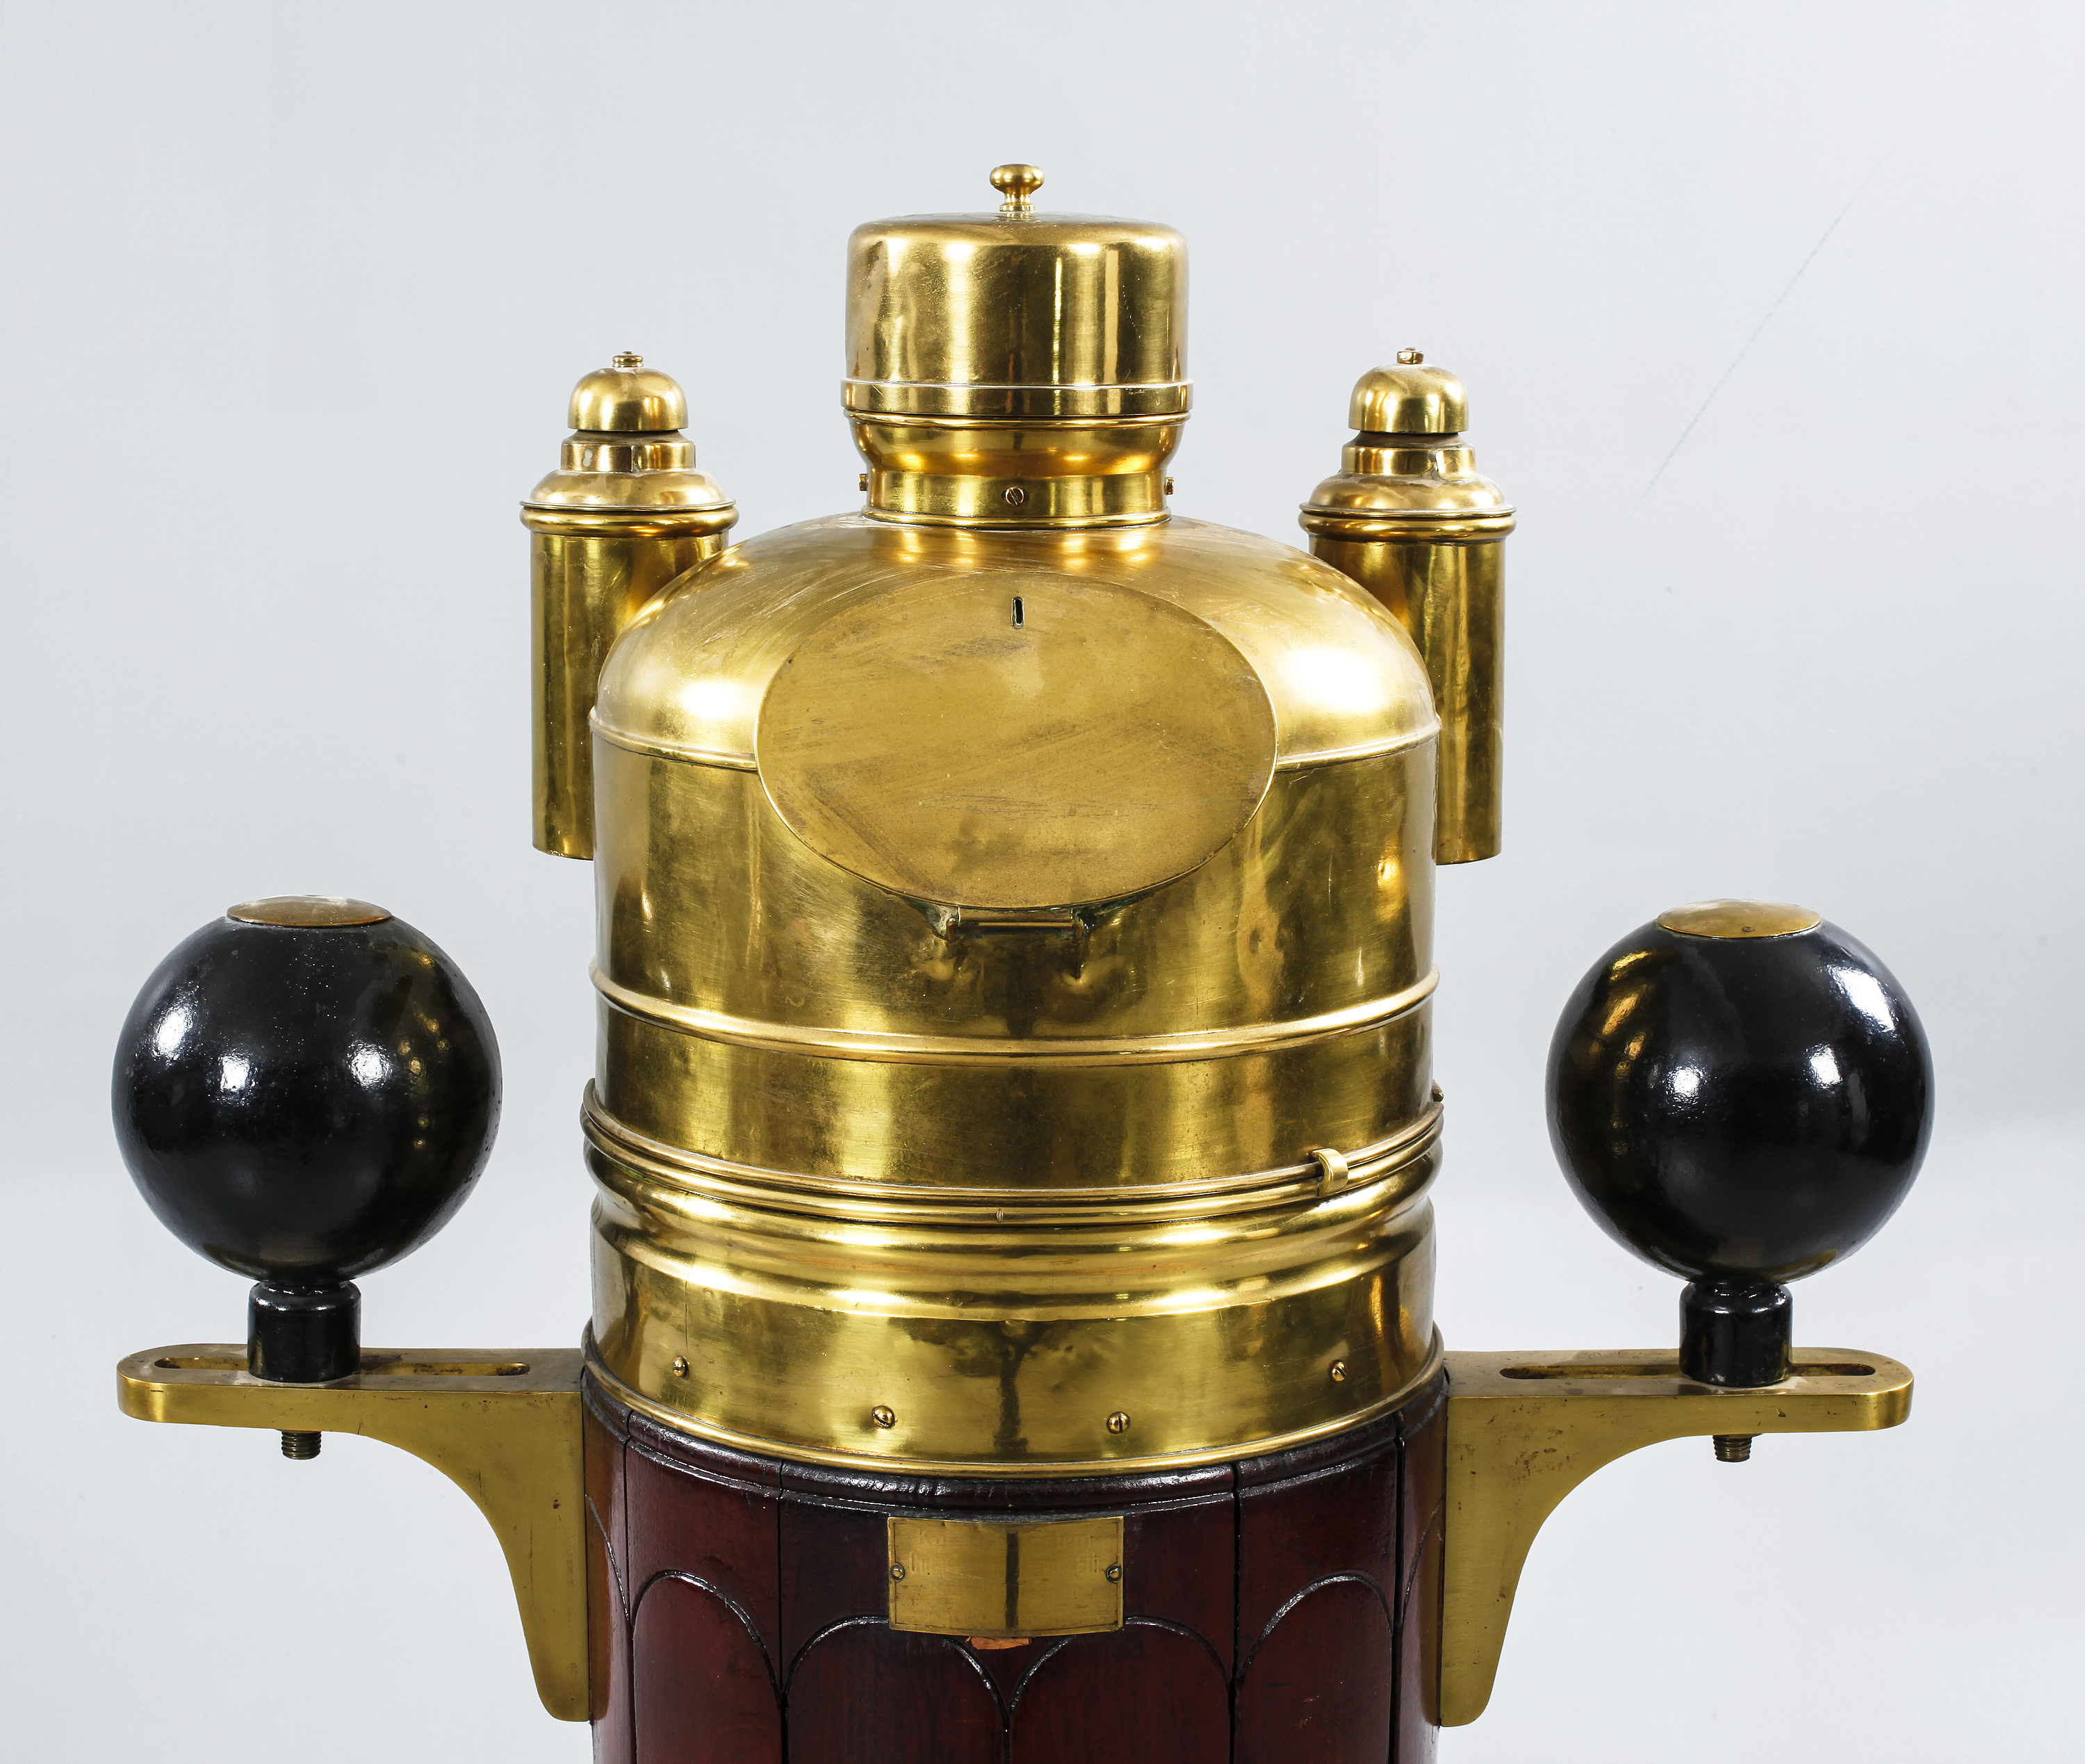
\includegraphics[scale=0.3]{Anh/ngoc2.jpg}
\end{center}

        Một hộp la bàn bảo vệ la bàn ở chính giữa, với hai quả cầu bằng sắt non để triệt tiêu phần bị lệch của la bàn, giúp la bàn quay đúng hướng. Việc sử dụng các quả cầu này được đề xuất bởi Lord Kelvin.

    Cũng như con tàu, các quả cầu sắt sẽ bị nhiễm từ do tác dụng của từ trường Trái Đất $B_e$. Là những quả cầu, chúng sẽ hoạt độn riên lẻ như các lưỡng cực. Một lưỡng cực có thể được coi như một trường tạo bởi hai đơn cực từ có moment từ $\pm m$ tại hai điểm khác nhau.
    Cảm ứng từ của một đơn cực từ là
    $$\ot{B}=\pm m\dfrac{\hat r}{r^2},$$
    Trong đó dấu dương tương ứng với cực bắc còn dấu âm tương ứng với cực nam. Từ trường của lưỡng cực là tổng hợp của hai trường: một của cực bắc tại $y=+a/2$ và một của cực nam tại $y=-a/2$, trong đó trục $y$ nằm ngang và hướng về phía bắc. $a$ là một khoảng cách nhỏ hơn rất nhiều so với bán kính các quả cầu; $a=K_iB_e$ trong đó $K_i$ là một hằng số phụ thuộc vào kích thước của các quả cầu sắt non.
    \begin{center}
        

\tikzset{every picture/.style={line width=0.75pt}} %set default line width to 0.75pt        

\begin{tikzpicture}[x=0.75pt,y=0.75pt,yscale=-1,xscale=1]
%uncomment if require: \path (0,466); %set diagram left start at 0, and has height of 466

%Shape: Circle [id:dp751806434667823] 
\draw   (98,277) .. controls (98,255.46) and (115.46,238) .. (137,238) .. controls (158.54,238) and (176,255.46) .. (176,277) .. controls (176,298.54) and (158.54,316) .. (137,316) .. controls (115.46,316) and (98,298.54) .. (98,277) -- cycle ;
%Straight Lines [id:da7958195415916756] 
\draw  [dash pattern={on 4.5pt off 4.5pt}]  (137,116) -- (137,284) ;
%Straight Lines [id:da11650011659130377] 
\draw  [dash pattern={on 4.5pt off 4.5pt}]  (137,277) -- (408,202) ;
%Straight Lines [id:da5651105007949573] 
\draw [line width=1.5]    (408,202) -- (466.27,224.56) ;
\draw [shift={(470,226)}, rotate = 201.16] [fill={rgb, 255:red, 0; green, 0; blue, 0 }  ][line width=0.08]  [draw opacity=0] (13.4,-6.43) -- (0,0) -- (13.4,6.44) -- (8.9,0) -- cycle    ;
%Shape: Circle [id:dp5068445005254147] 
\draw  [fill={rgb, 255:red, 0; green, 0; blue, 0 }  ,fill opacity=1 ] (132,262) .. controls (132,259.24) and (134.24,257) .. (137,257) .. controls (139.76,257) and (142,259.24) .. (142,262) .. controls (142,264.76) and (139.76,267) .. (137,267) .. controls (134.24,267) and (132,264.76) .. (132,262) -- cycle ;
%Shape: Circle [id:dp9877766218057484] 
\draw  [fill={rgb, 255:red, 0; green, 0; blue, 0 }  ,fill opacity=1 ] (132,289) .. controls (132,286.24) and (134.24,284) .. (137,284) .. controls (139.76,284) and (142,286.24) .. (142,289) .. controls (142,291.76) and (139.76,294) .. (137,294) .. controls (134.24,294) and (132,291.76) .. (132,289) -- cycle ;
%Straight Lines [id:da2796466001013038] 
\draw  [dash pattern={on 0.84pt off 2.51pt}]  (59,262) -- (137,262) ;
%Straight Lines [id:da8874709140465575] 
\draw  [dash pattern={on 0.84pt off 2.51pt}]  (59,289) -- (137,289) ;
%Straight Lines [id:da3482920020854341] 
\draw    (59,265) -- (59,289) ;
\draw [shift={(59,292)}, rotate = 270] [fill={rgb, 255:red, 0; green, 0; blue, 0 }  ][line width=0.08]  [draw opacity=0] (7.14,-3.43) -- (0,0) -- (7.14,3.43) -- (4.74,0) -- cycle    ;
\draw [shift={(59,262)}, rotate = 90] [fill={rgb, 255:red, 0; green, 0; blue, 0 }  ][line width=0.08]  [draw opacity=0] (7.14,-3.43) -- (0,0) -- (7.14,3.43) -- (4.74,0) -- cycle    ;

% Text Node
\draw (123,85.4) node [anchor=north west][inner sep=0.75pt]    {$\text{Bắc}$};
% Text Node
\draw (167,219.4) node [anchor=north west][inner sep=0.75pt]    {$\Phi $};
% Text Node
\draw (436,227.4) node [anchor=north west][inner sep=0.75pt]    {$\overrightarrow{B_{i}}$};
% Text Node
\draw (151,319.4) node [anchor=north west][inner sep=0.75pt]    {$\text{Bóng sắt}$};
% Text Node
\draw (37,267.4) node [anchor=north west][inner sep=0.75pt]    {$a$};


\end{tikzpicture}

    \end{center}
    \item Lập biểu thức cho từ trường $\ot{B_i}$ cách tâm quả cầu một khoảng $d\gg a$. Lưu ý rằng sẽ có một thành phần có phương hướng tâm, hướng ra quả cầu và một thành phần có phương tiếp tuyến với đường tròn bán kính $d$ xung quanh quả cầu, vì vậy nên sử dụng tọa độ cực.
    \item Nếu được đặt trực tiếp ở bên phải và trái của la bàn, các quả cầu sắt có thể được đặt ở khoảng cách $d$ để loại bỏ sai số từ tính cho các góc bất kì mà trong đó $\delta \theta$ là lớn nhất. Giả sử rằng điều này được thực hiện, tìm biểu thức cho góc lệch $\delta\theta$ do sự kết hợp hướng từ tính của con tàu và các quả cầu đối với góc $\theta$ bất kì.
\end{enumerate}

\end{vd}
\loigiai{
\begin{enumerate}[1)]
    \item Phân tích từ trường tổng hợp thành các từ trường thành phần. Thành phần từ trường hướng về phía Bắc là:
$$B_{\text{bắc}}=B_e-B_eK_b\cos\theta\cos\theta-B_eK_s\sin\theta\sin\theta,$$
trong khi đó thành phần hướng về phía Đông là:
$$B_{\text{đông}}=-B_3K_b\sin\theta\cos\theta+B_eK_s\cos\theta\sin\theta.$$
Ta được góc lệch:
$$ \tan \delta \theta=\left(K_{s}-K_{b}\right) \dfrac{\sin \theta \cos \theta}{1-K_{b} \cos ^{2} \theta-K_{s} \sin ^{2} \theta}.$$
Dạng của biểu thức này khá đẹp, vì như ta thấy, $K_b$ và $K_s$ đủ nhỏ để có thể bỏ qua ở mẫu.
    \item Bằng cách kiểm tra, ta thấy $\theta=45^\circ$ sẽ ứng với góc lệch lớn nhất. Và ta chấp nhận được các góc $45^\circ$, $135^\circ$, $225^\circ$ và $315^\circ$.
    \item Bài toán này không khó như ta nghĩ.\\
    \begin{center}
        

\tikzset{every picture/.style={line width=0.75pt}} %set default line width to 0.75pt        

\begin{tikzpicture}[x=0.75pt,y=0.75pt,yscale=-1,xscale=1]
%uncomment if require: \path (0,468); %set diagram left start at 0, and has height of 468

%Shape: Circle [id:dp283743452851426] 
\draw   (118,297) .. controls (118,275.46) and (135.46,258) .. (157,258) .. controls (178.54,258) and (196,275.46) .. (196,297) .. controls (196,318.54) and (178.54,336) .. (157,336) .. controls (135.46,336) and (118,318.54) .. (118,297) -- cycle ;
%Straight Lines [id:da9329698416959988] 
\draw  [dash pattern={on 4.5pt off 4.5pt}]  (157,136) -- (157,304) ;
%Shape: Circle [id:dp7302446853963502] 
\draw  [fill={rgb, 255:red, 0; green, 0; blue, 0 }  ,fill opacity=1 ] (152,282) .. controls (152,279.24) and (154.24,277) .. (157,277) .. controls (159.76,277) and (162,279.24) .. (162,282) .. controls (162,284.76) and (159.76,287) .. (157,287) .. controls (154.24,287) and (152,284.76) .. (152,282) -- cycle ;
%Shape: Circle [id:dp08946091539998635] 
\draw  [fill={rgb, 255:red, 0; green, 0; blue, 0 }  ,fill opacity=1 ] (152,309) .. controls (152,306.24) and (154.24,304) .. (157,304) .. controls (159.76,304) and (162,306.24) .. (162,309) .. controls (162,311.76) and (159.76,314) .. (157,314) .. controls (154.24,314) and (152,311.76) .. (152,309) -- cycle ;
%Straight Lines [id:da8503315996944931] 
\draw  [dash pattern={on 0.84pt off 2.51pt}]  (79,282) -- (157,282) ;
%Straight Lines [id:da4363280092273607] 
\draw  [dash pattern={on 0.84pt off 2.51pt}]  (79,309) -- (157,309) ;
%Straight Lines [id:da08272405117413917] 
\draw    (79,285) -- (79,309) ;
\draw [shift={(79,312)}, rotate = 270] [fill={rgb, 255:red, 0; green, 0; blue, 0 }  ][line width=0.08]  [draw opacity=0] (7.14,-3.43) -- (0,0) -- (7.14,3.43) -- (4.74,0) -- cycle    ;
\draw [shift={(79,282)}, rotate = 90] [fill={rgb, 255:red, 0; green, 0; blue, 0 }  ][line width=0.08]  [draw opacity=0] (7.14,-3.43) -- (0,0) -- (7.14,3.43) -- (4.74,0) -- cycle    ;
%Straight Lines [id:da016285889610417215] 
\draw [color={rgb, 255:red, 0; green, 0; blue, 0 }  ,draw opacity=1 ]   (157,282) -- (389,243) ;
%Straight Lines [id:da05152532762538198] 
\draw    (170.5,305) -- (389,243) ;
%Straight Lines [id:da8507054364259559] 
\draw [color={rgb, 255:red, 245; green, 166; blue, 35 }  ,draw opacity=1 ]   (391.89,242.18) -- (498,212) ;
\draw [shift={(389,243)}, rotate = 344.12] [fill={rgb, 255:red, 245; green, 166; blue, 35 }  ,fill opacity=1 ][line width=0.08]  [draw opacity=0] (10.72,-5.15) -- (0,0) -- (10.72,5.15) -- (7.12,0) -- cycle    ;
%Straight Lines [id:da4895425189234859] 
\draw [color={rgb, 255:red, 74; green, 144; blue, 226 }  ,draw opacity=1 ][fill={rgb, 255:red, 74; green, 144; blue, 226 }  ,fill opacity=1 ]   (389,243) -- (500.05,223.52) ;
\draw [shift={(503,223)}, rotate = 530.05] [fill={rgb, 255:red, 74; green, 144; blue, 226 }  ,fill opacity=1 ][line width=0.08]  [draw opacity=0] (10.72,-5.15) -- (0,0) -- (10.72,5.15) -- (7.12,0) -- cycle    ;
%Straight Lines [id:da05906959057280403] 
\draw [color={rgb, 255:red, 208; green, 2; blue, 27 }  ,draw opacity=1 ]   (159.5,283.5) -- (170.5,305) ;
%Straight Lines [id:da6543050515321556] 
\draw [color={rgb, 255:red, 79; green, 211; blue, 33 }  ,draw opacity=1 ]   (157,309) -- (170.5,305) ;

% Text Node
\draw (143,105.4) node [anchor=north west][inner sep=0.75pt]    {$\text{Bắc}$};
% Text Node
\draw (187,239.4) node [anchor=north west][inner sep=0.75pt]    {$\Phi $};
% Text Node
\draw (57,287.4) node [anchor=north west][inner sep=0.75pt]    {$a$};


\end{tikzpicture}

    \end{center}
    Xét hình tam giác màu ở trên. Cạnh màu đen có chiều dài $a$. Góc giữa cạnh màu xanh và đen là $\Phi$, nên chiều dài cạnh đỏ là $a\sin \Phi$ và chiều dài cạnh xanh là $a\cos \Phi$.\\
    Cảm ứng từ gây ra bởi một cực từ cách một khoảng $d$ là
    $$B=\pm m\dfrac{1}{d^2}.$$
    Tổng hợp của hai trường gồm có hai thành phần. Thành phần tiếp tuyến được tính bằng độ mở của tam giác tạo bởi hai vector, và vì hai vector có chiều dài xấp xỉ nhau, nên chúng ta có thể dùng biểu thức của tam giác đồng dạng:
    $$\dfrac{a \sin \phi}{d} \approx \dfrac{B_{\phi}}{B} \Rightarrow B_{\phi}=m \dfrac{a}{d^{3}} \sin \phi=B_{e} \dfrac{m K_{i}}{d^{3}} \sin \phi .$$
    Như mong đợi, thành phần này biến mất vì $\Phi=0$.\\
    Thành phần theo phương bán kính được xác định bởi sự khác biệt chiều dài của hai vector của hai trường, là:
    $$ B_{r}=m\left(\dfrac{1}{d^{2}}-\dfrac{1}{(d+x)^{2}}\right)=\dfrac{m}{d^{2}}\left(1-\dfrac{1}{(1+x / d)^{2}}\right) \approx \dfrac{m}{d^{2}} \dfrac{2 x}{d},$$
    trong đó $x=a\cos\Phi$ là chiều dài cạnh xanh lá, vì thế
    $$B_r=2B_e\dfrac{mK_i}{d^3}\cos\Phi.$$
    \item Lưu ý rằng từ trường gần la bàn do hai viên bi sắt tạo ra hoạt động khá giống với từ trường do cả con tàu. Thành phần hướng về phía mũi tàu là:
    $$B_b=-2B_{\theta} \propto \sin\Phi\propto\cos\theta,$$
    và thành phần hướng về mạn phải là:
    $$B_s=2B_r \propto \cos\Phi\propto\sin\theta,$$
    trong đó có thừa số $2$ bởi vì có hai quả cầu. Lưu ý rằng $\theta$ là hướng đi của con tàu trong khi $\Phi$ là góc hợp bởi cực Bắc và vị trí của la bàn so với một trong các quả cầu. Do đó, nếu như từ trường được hiệu chỉnh sao cho các góc tối đa, nó sẽ loại bỏ từ trường do tàu gây ra cho tất cả các góc, hay
    $$\delta \theta=0,$$
    với mọi $\theta$. Điều này có nghĩa là ta sẽ đặt vị trí các quả cầu sao cho $K_b=K_s$.
\end{enumerate}
}
\begin{vd}
Từ trường của Trái Đất là gần giống với một từ trường của một lưỡng cực từ. Ta có thể tưởng tượng có một lưỡng cực từ $\ot{m}$ ở tâm của Trái Đất. Để đơn giản, giả sử rằng $\ot{m}$ nằm trên trục quay của Trái Đất, hướng từ Bắc vào Nam, như hình vẽ. Hồng Kông nằm ở vĩ độ $\alpha=22^\circ$. Từ trường tại điểm cách lưỡng cực từ một khoảng là $\ot{r}$ được tính theo công thức
\[\ot{B}=\dfrac{\mu_o}{4\pi}\left[\dfrac{3(\ot{m}\cdot\ot{r})\ot{r}}{r^3}-\dfrac{\ot{m}}{r^3}\right]\]
\begin{enumerate}[1) ]
    \item Tìm hướng của từ trường tại Hồng Kông theo các phía Đông, Tây, Bắc, Nam, và các góc hợp với mặt ngang.
    \item Một dây điện nằm ngang có chiều dài $10~\mathrm{m}$, mang dòng điện có cường độ $100~\mathrm{A}$ theo hướng Bắc $-$ Nam. Tìm lực từ tác dụng lên dây. (Bạn cần phải nhớ độ lớn của từ trường Trái Đất trên bề mặt Trái Đất).
\end{enumerate}
\begin{center}
    

\tikzset{every picture/.style={line width=0.75pt}} %set default line width to 0.75pt        

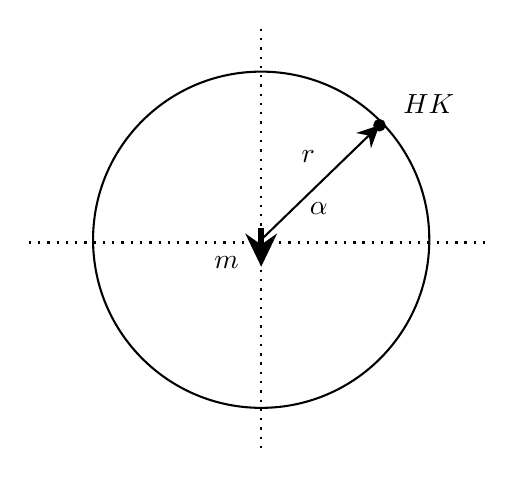
\begin{tikzpicture}[x=0.75pt,y=0.75pt,yscale=-1,xscale=1]
%uncomment if require: \path (0,300); %set diagram left start at 0, and has height of 300

%Shape: Circle [id:dp12955050763248477] 
\draw   (239,169) .. controls (239,124.26) and (275.26,88) .. (320,88) .. controls (364.74,88) and (401,124.26) .. (401,169) .. controls (401,213.74) and (364.74,250) .. (320,250) .. controls (275.26,250) and (239,213.74) .. (239,169) -- cycle ;
%Straight Lines [id:da33432597677839704] 
\draw  [dash pattern={on 0.84pt off 2.51pt}]  (208,170.33) -- (428,170.33) ;
%Straight Lines [id:da6659306133043119] 
\draw  [dash pattern={on 0.84pt off 2.51pt}]  (320,67.33) -- (320,270.33) ;
%Straight Lines [id:da013535855620636417] 
\draw    (320,169) -- (374.84,115.92) ;
\draw [shift={(377,113.83)}, rotate = 495.94] [fill={rgb, 255:red, 0; green, 0; blue, 0 }  ][line width=0.08]  [draw opacity=0] (10.72,-5.15) -- (0,0) -- (10.72,5.15) -- (7.12,0) -- cycle    ;
%Shape: Circle [id:dp570580867637053] 
\draw  [fill={rgb, 255:red, 0; green, 0; blue, 0 }  ,fill opacity=1 ] (379.5,113.83) .. controls (379.5,112.45) and (378.38,111.33) .. (377,111.33) .. controls (375.62,111.33) and (374.5,112.45) .. (374.5,113.83) .. controls (374.5,115.21) and (375.62,116.33) .. (377,116.33) .. controls (378.38,116.33) and (379.5,115.21) .. (379.5,113.83) -- cycle ;
%Straight Lines [id:da7218913590835949] 
\draw [line width=2.25]    (320,163.33) -- (320,177) ;
\draw [shift={(320,182)}, rotate = 270] [fill={rgb, 255:red, 0; green, 0; blue, 0 }  ][line width=0.08]  [draw opacity=0] (16.07,-7.72) -- (0,0) -- (16.07,7.72) -- (10.67,0) -- cycle    ;

% Text Node
\draw (338,124.4) node [anchor=north west][inner sep=0.75pt]    {$\ot{r}$};
% Text Node
\draw (296,175.4) node [anchor=north west][inner sep=0.75pt]    {$\ot{m}$};
% Text Node
\draw (342,149.4) node [anchor=north west][inner sep=0.75pt]    {$\alpha $};
% Text Node
\draw (387,97.4) node [anchor=north west][inner sep=0.75pt]    {$HK$};


\end{tikzpicture}
\end{center}
\end{vd}
\begin{loigiai}
\begin{enumerate}[1) ]
    \item 
    \begin{align*}
        \ot{B}&=\dfrac{\mu_0}{4\pi}\dfrac{1}{r^3}\left[3(\ot{m}\cdot\ot{r})\ot{r}-\ot{m}\right]\\
        &=\dfrac{\mu_0}{4\pi}\dfrac{1}{R^3}\left[3((-m\cdot\ot{z})\cdot\ot{r})\ot{r}-(-m)\ot{z}\right]\\
        &=\dfrac{\mu_0}{4\pi}\dfrac{m}{R^3}\left[-3\mathrm{\sin{\alpha}}\cdot\ot{r}+\left(\mathrm{\sin{\alpha}}\cdot\ot{r}-\mathrm{\cos{\alpha}}\cdot\ot{\theta}\right)\right]\\
        &=\dfrac{\mu_0}{4\pi}\dfrac{m}{R^3}\left[-2\mathrm{\sin{\alpha}}\cdot\ot{r}-\mathrm{\cos{\alpha}}\cdot\ot{\theta}\right].
    \end{align*}
    Từ Bắc tới Nam, tại góc $\beta=2\mathrm{\arctan{(2\mathrm{\tan{\alpha}})}}=38,9^\circ$ chỉ hướng xuống.
    \item $\left|\ot{B}\right|\cong0,5\cdot10^{-4}~\mathrm{T}$.
    Và độ lớn của lực từ là:
    \[\left|\ot{F}\right|=I\left|\ot{\ell}\times\ot{B}\right|=IB\ell\mathrm{\sin{\theta}}=0,0315~\mathrm{N}.\]
\end{enumerate}
\end{loigiai}